% Created by tikzDevice version 0.12 on 2019-03-22 14:21:41
% !TEX encoding = UTF-8 Unicode
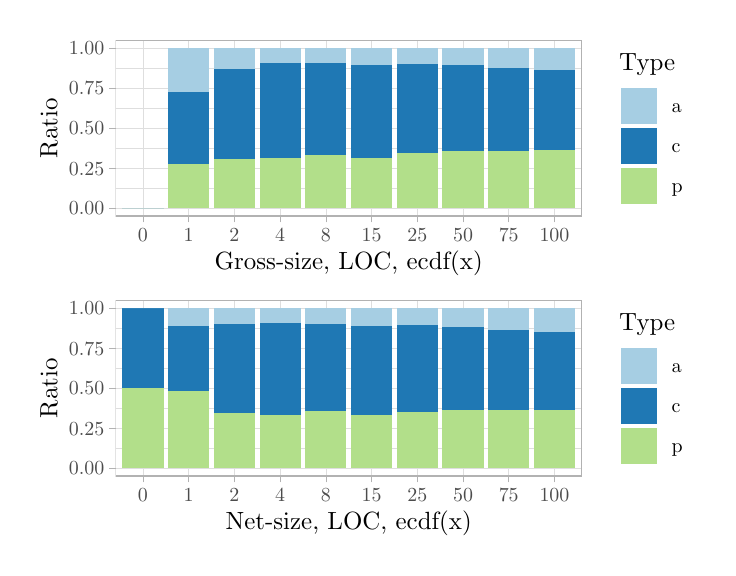
\begin{tikzpicture}[x=1pt,y=1pt]
\definecolor{fillColor}{RGB}{255,255,255}
\path[use as bounding box,fill=fillColor,fill opacity=0.00] (0,0) rectangle (245.72,187.90);
\begin{scope}
\path[clip] (  0.00, 93.95) rectangle (245.72,187.90);
\definecolor{drawColor}{RGB}{255,255,255}
\definecolor{fillColor}{RGB}{255,255,255}

\path[draw=drawColor,line width= 0.5pt,line join=round,line cap=round,fill=fillColor] (  0.00, 93.95) rectangle (245.72,187.90);
\end{scope}
\begin{scope}
\path[clip] ( 31.74,119.80) rectangle (200.26,183.40);
\definecolor{fillColor}{RGB}{255,255,255}

\path[fill=fillColor] ( 31.74,119.80) rectangle (200.26,183.40);
\definecolor{drawColor}{gray}{0.87}

\path[draw=drawColor,line width= 0.1pt,line join=round] ( 31.74,129.92) --
	(200.26,129.92);

\path[draw=drawColor,line width= 0.1pt,line join=round] ( 31.74,144.37) --
	(200.26,144.37);

\path[draw=drawColor,line width= 0.1pt,line join=round] ( 31.74,158.83) --
	(200.26,158.83);

\path[draw=drawColor,line width= 0.1pt,line join=round] ( 31.74,173.28) --
	(200.26,173.28);

\path[draw=drawColor,line width= 0.2pt,line join=round] ( 31.74,122.69) --
	(200.26,122.69);

\path[draw=drawColor,line width= 0.2pt,line join=round] ( 31.74,137.14) --
	(200.26,137.14);

\path[draw=drawColor,line width= 0.2pt,line join=round] ( 31.74,151.60) --
	(200.26,151.60);

\path[draw=drawColor,line width= 0.2pt,line join=round] ( 31.74,166.05) --
	(200.26,166.05);

\path[draw=drawColor,line width= 0.2pt,line join=round] ( 31.74,180.51) --
	(200.26,180.51);

\path[draw=drawColor,line width= 0.2pt,line join=round] ( 41.65,119.80) --
	( 41.65,183.40);

\path[draw=drawColor,line width= 0.2pt,line join=round] ( 58.17,119.80) --
	( 58.17,183.40);

\path[draw=drawColor,line width= 0.2pt,line join=round] ( 74.70,119.80) --
	( 74.70,183.40);

\path[draw=drawColor,line width= 0.2pt,line join=round] ( 91.22,119.80) --
	( 91.22,183.40);

\path[draw=drawColor,line width= 0.2pt,line join=round] (107.74,119.80) --
	(107.74,183.40);

\path[draw=drawColor,line width= 0.2pt,line join=round] (124.26,119.80) --
	(124.26,183.40);

\path[draw=drawColor,line width= 0.2pt,line join=round] (140.79,119.80) --
	(140.79,183.40);

\path[draw=drawColor,line width= 0.2pt,line join=round] (157.31,119.80) --
	(157.31,183.40);

\path[draw=drawColor,line width= 0.2pt,line join=round] (173.83,119.80) --
	(173.83,183.40);

\path[draw=drawColor,line width= 0.2pt,line join=round] (190.35,119.80) --
	(190.35,183.40);
\definecolor{fillColor}{RGB}{178,223,138}

\path[fill=fillColor] ( 34.22,122.69) rectangle ( 49.09,122.69);
\definecolor{fillColor}{RGB}{31,120,180}

\path[fill=fillColor] ( 34.22,122.69) rectangle ( 49.09,122.69);
\definecolor{fillColor}{RGB}{166,206,227}

\path[fill=fillColor] ( 34.22,122.69) rectangle ( 49.09,122.69);
\definecolor{fillColor}{RGB}{178,223,138}

\path[fill=fillColor] ( 50.74,122.69) rectangle ( 65.61,138.46);
\definecolor{fillColor}{RGB}{31,120,180}

\path[fill=fillColor] ( 50.74,138.46) rectangle ( 65.61,164.74);
\definecolor{fillColor}{RGB}{166,206,227}

\path[fill=fillColor] ( 50.74,164.74) rectangle ( 65.61,180.51);
\definecolor{fillColor}{RGB}{178,223,138}

\path[fill=fillColor] ( 67.26,122.69) rectangle ( 82.13,140.29);
\definecolor{fillColor}{RGB}{31,120,180}

\path[fill=fillColor] ( 67.26,140.29) rectangle ( 82.13,172.97);
\definecolor{fillColor}{RGB}{166,206,227}

\path[fill=fillColor] ( 67.26,172.97) rectangle ( 82.13,180.51);
\definecolor{fillColor}{RGB}{178,223,138}

\path[fill=fillColor] ( 83.78,122.69) rectangle ( 98.65,140.92);
\definecolor{fillColor}{RGB}{31,120,180}

\path[fill=fillColor] ( 83.78,140.92) rectangle ( 98.65,175.17);
\definecolor{fillColor}{RGB}{166,206,227}

\path[fill=fillColor] ( 83.78,175.17) rectangle ( 98.65,180.51);
\definecolor{fillColor}{RGB}{178,223,138}

\path[fill=fillColor] (100.31,122.69) rectangle (115.18,141.87);
\definecolor{fillColor}{RGB}{31,120,180}

\path[fill=fillColor] (100.31,141.87) rectangle (115.18,175.25);
\definecolor{fillColor}{RGB}{166,206,227}

\path[fill=fillColor] (100.31,175.25) rectangle (115.18,180.51);
\definecolor{fillColor}{RGB}{178,223,138}

\path[fill=fillColor] (116.83,122.69) rectangle (131.70,140.83);
\definecolor{fillColor}{RGB}{31,120,180}

\path[fill=fillColor] (116.83,140.83) rectangle (131.70,174.24);
\definecolor{fillColor}{RGB}{166,206,227}

\path[fill=fillColor] (116.83,174.24) rectangle (131.70,180.51);
\definecolor{fillColor}{RGB}{178,223,138}

\path[fill=fillColor] (133.35,122.69) rectangle (148.22,142.44);
\definecolor{fillColor}{RGB}{31,120,180}

\path[fill=fillColor] (133.35,142.44) rectangle (148.22,174.75);
\definecolor{fillColor}{RGB}{166,206,227}

\path[fill=fillColor] (133.35,174.75) rectangle (148.22,180.51);
\definecolor{fillColor}{RGB}{178,223,138}

\path[fill=fillColor] (149.87,122.69) rectangle (164.74,143.37);
\definecolor{fillColor}{RGB}{31,120,180}

\path[fill=fillColor] (149.87,143.37) rectangle (164.74,174.38);
\definecolor{fillColor}{RGB}{166,206,227}

\path[fill=fillColor] (149.87,174.38) rectangle (164.74,180.51);
\definecolor{fillColor}{RGB}{178,223,138}

\path[fill=fillColor] (166.39,122.69) rectangle (181.26,143.43);
\definecolor{fillColor}{RGB}{31,120,180}

\path[fill=fillColor] (166.39,143.43) rectangle (181.26,173.27);
\definecolor{fillColor}{RGB}{166,206,227}

\path[fill=fillColor] (166.39,173.27) rectangle (181.26,180.51);
\definecolor{fillColor}{RGB}{178,223,138}

\path[fill=fillColor] (182.92,122.69) rectangle (197.79,143.52);
\definecolor{fillColor}{RGB}{31,120,180}

\path[fill=fillColor] (182.92,143.52) rectangle (197.79,172.77);
\definecolor{fillColor}{RGB}{166,206,227}

\path[fill=fillColor] (182.92,172.77) rectangle (197.79,180.51);
\definecolor{drawColor}{gray}{0.70}

\path[draw=drawColor,line width= 0.5pt,line join=round,line cap=round] ( 31.74,119.80) rectangle (200.26,183.40);
\end{scope}
\begin{scope}
\path[clip] (  0.00,  0.00) rectangle (245.72,187.90);
\definecolor{drawColor}{gray}{0.30}

\node[text=drawColor,anchor=base east,inner sep=0pt, outer sep=0pt, scale=  0.72] at ( 27.69,120.21) {0.00};

\node[text=drawColor,anchor=base east,inner sep=0pt, outer sep=0pt, scale=  0.72] at ( 27.69,134.66) {0.25};

\node[text=drawColor,anchor=base east,inner sep=0pt, outer sep=0pt, scale=  0.72] at ( 27.69,149.12) {0.50};

\node[text=drawColor,anchor=base east,inner sep=0pt, outer sep=0pt, scale=  0.72] at ( 27.69,163.58) {0.75};

\node[text=drawColor,anchor=base east,inner sep=0pt, outer sep=0pt, scale=  0.72] at ( 27.69,178.03) {1.00};
\end{scope}
\begin{scope}
\path[clip] (  0.00,  0.00) rectangle (245.72,187.90);
\definecolor{drawColor}{gray}{0.70}

\path[draw=drawColor,line width= 0.2pt,line join=round] ( 29.49,122.69) --
	( 31.74,122.69);

\path[draw=drawColor,line width= 0.2pt,line join=round] ( 29.49,137.14) --
	( 31.74,137.14);

\path[draw=drawColor,line width= 0.2pt,line join=round] ( 29.49,151.60) --
	( 31.74,151.60);

\path[draw=drawColor,line width= 0.2pt,line join=round] ( 29.49,166.05) --
	( 31.74,166.05);

\path[draw=drawColor,line width= 0.2pt,line join=round] ( 29.49,180.51) --
	( 31.74,180.51);
\end{scope}
\begin{scope}
\path[clip] (  0.00,  0.00) rectangle (245.72,187.90);
\definecolor{drawColor}{gray}{0.70}

\path[draw=drawColor,line width= 0.2pt,line join=round] ( 41.65,117.55) --
	( 41.65,119.80);

\path[draw=drawColor,line width= 0.2pt,line join=round] ( 58.17,117.55) --
	( 58.17,119.80);

\path[draw=drawColor,line width= 0.2pt,line join=round] ( 74.70,117.55) --
	( 74.70,119.80);

\path[draw=drawColor,line width= 0.2pt,line join=round] ( 91.22,117.55) --
	( 91.22,119.80);

\path[draw=drawColor,line width= 0.2pt,line join=round] (107.74,117.55) --
	(107.74,119.80);

\path[draw=drawColor,line width= 0.2pt,line join=round] (124.26,117.55) --
	(124.26,119.80);

\path[draw=drawColor,line width= 0.2pt,line join=round] (140.79,117.55) --
	(140.79,119.80);

\path[draw=drawColor,line width= 0.2pt,line join=round] (157.31,117.55) --
	(157.31,119.80);

\path[draw=drawColor,line width= 0.2pt,line join=round] (173.83,117.55) --
	(173.83,119.80);

\path[draw=drawColor,line width= 0.2pt,line join=round] (190.35,117.55) --
	(190.35,119.80);
\end{scope}
\begin{scope}
\path[clip] (  0.00,  0.00) rectangle (245.72,187.90);
\definecolor{drawColor}{gray}{0.30}

\node[text=drawColor,anchor=base,inner sep=0pt, outer sep=0pt, scale=  0.72] at ( 41.65,110.79) {0};

\node[text=drawColor,anchor=base,inner sep=0pt, outer sep=0pt, scale=  0.72] at ( 58.17,110.79) {1};

\node[text=drawColor,anchor=base,inner sep=0pt, outer sep=0pt, scale=  0.72] at ( 74.70,110.79) {2};

\node[text=drawColor,anchor=base,inner sep=0pt, outer sep=0pt, scale=  0.72] at ( 91.22,110.79) {4};

\node[text=drawColor,anchor=base,inner sep=0pt, outer sep=0pt, scale=  0.72] at (107.74,110.79) {8};

\node[text=drawColor,anchor=base,inner sep=0pt, outer sep=0pt, scale=  0.72] at (124.26,110.79) {15};

\node[text=drawColor,anchor=base,inner sep=0pt, outer sep=0pt, scale=  0.72] at (140.79,110.79) {25};

\node[text=drawColor,anchor=base,inner sep=0pt, outer sep=0pt, scale=  0.72] at (157.31,110.79) {50};

\node[text=drawColor,anchor=base,inner sep=0pt, outer sep=0pt, scale=  0.72] at (173.83,110.79) {75};

\node[text=drawColor,anchor=base,inner sep=0pt, outer sep=0pt, scale=  0.72] at (190.35,110.79) {100};
\end{scope}
\begin{scope}
\path[clip] (  0.00,  0.00) rectangle (245.72,187.90);
\definecolor{drawColor}{RGB}{0,0,0}

\node[text=drawColor,anchor=base,inner sep=0pt, outer sep=0pt, scale=  0.90] at (116.00,100.39) {Gross-size, LOC, ecdf(x)};
\end{scope}
\begin{scope}
\path[clip] (  0.00,  0.00) rectangle (245.72,187.90);
\definecolor{drawColor}{RGB}{0,0,0}

\node[text=drawColor,rotate= 90.00,anchor=base,inner sep=0pt, outer sep=0pt, scale=  0.90] at ( 10.70,151.60) {Ratio};
\end{scope}
\begin{scope}
\path[clip] (  0.00,  0.00) rectangle (245.72,187.90);
\definecolor{fillColor}{RGB}{255,255,255}

\path[fill=fillColor] (209.26,119.10) rectangle (241.22,184.10);
\end{scope}
\begin{scope}
\path[clip] (  0.00,  0.00) rectangle (245.72,187.90);
\definecolor{drawColor}{RGB}{0,0,0}

\node[text=drawColor,anchor=base west,inner sep=0pt, outer sep=0pt, scale=  0.90] at (213.76,172.43) {Type};
\end{scope}
\begin{scope}
\path[clip] (  0.00,  0.00) rectangle (245.72,187.90);
\definecolor{fillColor}{RGB}{255,255,255}

\path[fill=fillColor] (213.76,152.50) rectangle (228.22,166.96);
\end{scope}
\begin{scope}
\path[clip] (  0.00,  0.00) rectangle (245.72,187.90);
\definecolor{fillColor}{RGB}{166,206,227}

\path[fill=fillColor] (214.48,153.22) rectangle (227.51,166.25);
\end{scope}
\begin{scope}
\path[clip] (  0.00,  0.00) rectangle (245.72,187.90);
\definecolor{fillColor}{RGB}{255,255,255}

\path[fill=fillColor] (213.76,138.05) rectangle (228.22,152.50);
\end{scope}
\begin{scope}
\path[clip] (  0.00,  0.00) rectangle (245.72,187.90);
\definecolor{fillColor}{RGB}{31,120,180}

\path[fill=fillColor] (214.48,138.76) rectangle (227.51,151.79);
\end{scope}
\begin{scope}
\path[clip] (  0.00,  0.00) rectangle (245.72,187.90);
\definecolor{fillColor}{RGB}{255,255,255}

\path[fill=fillColor] (213.76,123.60) rectangle (228.22,138.05);
\end{scope}
\begin{scope}
\path[clip] (  0.00,  0.00) rectangle (245.72,187.90);
\definecolor{fillColor}{RGB}{178,223,138}

\path[fill=fillColor] (214.48,124.31) rectangle (227.51,137.34);
\end{scope}
\begin{scope}
\path[clip] (  0.00,  0.00) rectangle (245.72,187.90);
\definecolor{drawColor}{RGB}{0,0,0}

\node[text=drawColor,anchor=base west,inner sep=0pt, outer sep=0pt, scale=  0.72] at (232.72,157.25) {a};
\end{scope}
\begin{scope}
\path[clip] (  0.00,  0.00) rectangle (245.72,187.90);
\definecolor{drawColor}{RGB}{0,0,0}

\node[text=drawColor,anchor=base west,inner sep=0pt, outer sep=0pt, scale=  0.72] at (232.72,142.80) {c};
\end{scope}
\begin{scope}
\path[clip] (  0.00,  0.00) rectangle (245.72,187.90);
\definecolor{drawColor}{RGB}{0,0,0}

\node[text=drawColor,anchor=base west,inner sep=0pt, outer sep=0pt, scale=  0.72] at (232.72,128.34) {p};
\end{scope}
\begin{scope}
\path[clip] (  0.00,  0.00) rectangle (245.72, 93.95);
\definecolor{drawColor}{RGB}{255,255,255}
\definecolor{fillColor}{RGB}{255,255,255}

\path[draw=drawColor,line width= 0.5pt,line join=round,line cap=round,fill=fillColor] (  0.00,  0.00) rectangle (245.72, 93.95);
\end{scope}
\begin{scope}
\path[clip] ( 31.74, 25.85) rectangle (200.26, 89.45);
\definecolor{fillColor}{RGB}{255,255,255}

\path[fill=fillColor] ( 31.74, 25.85) rectangle (200.26, 89.45);
\definecolor{drawColor}{gray}{0.87}

\path[draw=drawColor,line width= 0.1pt,line join=round] ( 31.74, 35.96) --
	(200.26, 35.96);

\path[draw=drawColor,line width= 0.1pt,line join=round] ( 31.74, 50.42) --
	(200.26, 50.42);

\path[draw=drawColor,line width= 0.1pt,line join=round] ( 31.74, 64.88) --
	(200.26, 64.88);

\path[draw=drawColor,line width= 0.1pt,line join=round] ( 31.74, 79.33) --
	(200.26, 79.33);

\path[draw=drawColor,line width= 0.2pt,line join=round] ( 31.74, 28.74) --
	(200.26, 28.74);

\path[draw=drawColor,line width= 0.2pt,line join=round] ( 31.74, 43.19) --
	(200.26, 43.19);

\path[draw=drawColor,line width= 0.2pt,line join=round] ( 31.74, 57.65) --
	(200.26, 57.65);

\path[draw=drawColor,line width= 0.2pt,line join=round] ( 31.74, 72.10) --
	(200.26, 72.10);

\path[draw=drawColor,line width= 0.2pt,line join=round] ( 31.74, 86.56) --
	(200.26, 86.56);

\path[draw=drawColor,line width= 0.2pt,line join=round] ( 41.65, 25.85) --
	( 41.65, 89.45);

\path[draw=drawColor,line width= 0.2pt,line join=round] ( 58.17, 25.85) --
	( 58.17, 89.45);

\path[draw=drawColor,line width= 0.2pt,line join=round] ( 74.70, 25.85) --
	( 74.70, 89.45);

\path[draw=drawColor,line width= 0.2pt,line join=round] ( 91.22, 25.85) --
	( 91.22, 89.45);

\path[draw=drawColor,line width= 0.2pt,line join=round] (107.74, 25.85) --
	(107.74, 89.45);

\path[draw=drawColor,line width= 0.2pt,line join=round] (124.26, 25.85) --
	(124.26, 89.45);

\path[draw=drawColor,line width= 0.2pt,line join=round] (140.79, 25.85) --
	(140.79, 89.45);

\path[draw=drawColor,line width= 0.2pt,line join=round] (157.31, 25.85) --
	(157.31, 89.45);

\path[draw=drawColor,line width= 0.2pt,line join=round] (173.83, 25.85) --
	(173.83, 89.45);

\path[draw=drawColor,line width= 0.2pt,line join=round] (190.35, 25.85) --
	(190.35, 89.45);
\definecolor{fillColor}{RGB}{178,223,138}

\path[fill=fillColor] ( 34.22, 28.74) rectangle ( 49.09, 57.65);
\definecolor{fillColor}{RGB}{31,120,180}

\path[fill=fillColor] ( 34.22, 57.65) rectangle ( 49.09, 86.56);
\definecolor{fillColor}{RGB}{166,206,227}

\path[fill=fillColor] ( 34.22, 86.56) rectangle ( 49.09, 86.56);
\definecolor{fillColor}{RGB}{178,223,138}

\path[fill=fillColor] ( 50.74, 28.74) rectangle ( 65.61, 56.58);
\definecolor{fillColor}{RGB}{31,120,180}

\path[fill=fillColor] ( 50.74, 56.58) rectangle ( 65.61, 80.13);
\definecolor{fillColor}{RGB}{166,206,227}

\path[fill=fillColor] ( 50.74, 80.13) rectangle ( 65.61, 86.56);
\definecolor{fillColor}{RGB}{178,223,138}

\path[fill=fillColor] ( 67.26, 28.74) rectangle ( 82.13, 48.65);
\definecolor{fillColor}{RGB}{31,120,180}

\path[fill=fillColor] ( 67.26, 48.65) rectangle ( 82.13, 80.78);
\definecolor{fillColor}{RGB}{166,206,227}

\path[fill=fillColor] ( 67.26, 80.78) rectangle ( 82.13, 86.56);
\definecolor{fillColor}{RGB}{178,223,138}

\path[fill=fillColor] ( 83.78, 28.74) rectangle ( 98.65, 48.01);
\definecolor{fillColor}{RGB}{31,120,180}

\path[fill=fillColor] ( 83.78, 48.01) rectangle ( 98.65, 81.21);
\definecolor{fillColor}{RGB}{166,206,227}

\path[fill=fillColor] ( 83.78, 81.21) rectangle ( 98.65, 86.56);
\definecolor{fillColor}{RGB}{178,223,138}

\path[fill=fillColor] (100.31, 28.74) rectangle (115.18, 49.37);
\definecolor{fillColor}{RGB}{31,120,180}

\path[fill=fillColor] (100.31, 49.37) rectangle (115.18, 80.89);
\definecolor{fillColor}{RGB}{166,206,227}

\path[fill=fillColor] (100.31, 80.89) rectangle (115.18, 86.56);
\definecolor{fillColor}{RGB}{178,223,138}

\path[fill=fillColor] (116.83, 28.74) rectangle (131.70, 47.76);
\definecolor{fillColor}{RGB}{31,120,180}

\path[fill=fillColor] (116.83, 47.76) rectangle (131.70, 80.12);
\definecolor{fillColor}{RGB}{166,206,227}

\path[fill=fillColor] (116.83, 80.12) rectangle (131.70, 86.56);
\definecolor{fillColor}{RGB}{178,223,138}

\path[fill=fillColor] (133.35, 28.74) rectangle (148.22, 48.85);
\definecolor{fillColor}{RGB}{31,120,180}

\path[fill=fillColor] (133.35, 48.85) rectangle (148.22, 80.39);
\definecolor{fillColor}{RGB}{166,206,227}

\path[fill=fillColor] (133.35, 80.39) rectangle (148.22, 86.56);
\definecolor{fillColor}{RGB}{178,223,138}

\path[fill=fillColor] (149.87, 28.74) rectangle (164.74, 49.83);
\definecolor{fillColor}{RGB}{31,120,180}

\path[fill=fillColor] (149.87, 49.83) rectangle (164.74, 79.73);
\definecolor{fillColor}{RGB}{166,206,227}

\path[fill=fillColor] (149.87, 79.73) rectangle (164.74, 86.56);
\definecolor{fillColor}{RGB}{178,223,138}

\path[fill=fillColor] (166.39, 28.74) rectangle (181.26, 49.86);
\definecolor{fillColor}{RGB}{31,120,180}

\path[fill=fillColor] (166.39, 49.86) rectangle (181.26, 78.48);
\definecolor{fillColor}{RGB}{166,206,227}

\path[fill=fillColor] (166.39, 78.48) rectangle (181.26, 86.56);
\definecolor{fillColor}{RGB}{178,223,138}

\path[fill=fillColor] (182.92, 28.74) rectangle (197.79, 49.66);
\definecolor{fillColor}{RGB}{31,120,180}

\path[fill=fillColor] (182.92, 49.66) rectangle (197.79, 77.75);
\definecolor{fillColor}{RGB}{166,206,227}

\path[fill=fillColor] (182.92, 77.75) rectangle (197.79, 86.56);
\definecolor{drawColor}{gray}{0.70}

\path[draw=drawColor,line width= 0.5pt,line join=round,line cap=round] ( 31.74, 25.85) rectangle (200.26, 89.45);
\end{scope}
\begin{scope}
\path[clip] (  0.00,  0.00) rectangle (245.72,187.90);
\definecolor{drawColor}{gray}{0.30}

\node[text=drawColor,anchor=base east,inner sep=0pt, outer sep=0pt, scale=  0.72] at ( 27.69, 26.26) {0.00};

\node[text=drawColor,anchor=base east,inner sep=0pt, outer sep=0pt, scale=  0.72] at ( 27.69, 40.71) {0.25};

\node[text=drawColor,anchor=base east,inner sep=0pt, outer sep=0pt, scale=  0.72] at ( 27.69, 55.17) {0.50};

\node[text=drawColor,anchor=base east,inner sep=0pt, outer sep=0pt, scale=  0.72] at ( 27.69, 69.62) {0.75};

\node[text=drawColor,anchor=base east,inner sep=0pt, outer sep=0pt, scale=  0.72] at ( 27.69, 84.08) {1.00};
\end{scope}
\begin{scope}
\path[clip] (  0.00,  0.00) rectangle (245.72,187.90);
\definecolor{drawColor}{gray}{0.70}

\path[draw=drawColor,line width= 0.2pt,line join=round] ( 29.49, 28.74) --
	( 31.74, 28.74);

\path[draw=drawColor,line width= 0.2pt,line join=round] ( 29.49, 43.19) --
	( 31.74, 43.19);

\path[draw=drawColor,line width= 0.2pt,line join=round] ( 29.49, 57.65) --
	( 31.74, 57.65);

\path[draw=drawColor,line width= 0.2pt,line join=round] ( 29.49, 72.10) --
	( 31.74, 72.10);

\path[draw=drawColor,line width= 0.2pt,line join=round] ( 29.49, 86.56) --
	( 31.74, 86.56);
\end{scope}
\begin{scope}
\path[clip] (  0.00,  0.00) rectangle (245.72,187.90);
\definecolor{drawColor}{gray}{0.70}

\path[draw=drawColor,line width= 0.2pt,line join=round] ( 41.65, 23.60) --
	( 41.65, 25.85);

\path[draw=drawColor,line width= 0.2pt,line join=round] ( 58.17, 23.60) --
	( 58.17, 25.85);

\path[draw=drawColor,line width= 0.2pt,line join=round] ( 74.70, 23.60) --
	( 74.70, 25.85);

\path[draw=drawColor,line width= 0.2pt,line join=round] ( 91.22, 23.60) --
	( 91.22, 25.85);

\path[draw=drawColor,line width= 0.2pt,line join=round] (107.74, 23.60) --
	(107.74, 25.85);

\path[draw=drawColor,line width= 0.2pt,line join=round] (124.26, 23.60) --
	(124.26, 25.85);

\path[draw=drawColor,line width= 0.2pt,line join=round] (140.79, 23.60) --
	(140.79, 25.85);

\path[draw=drawColor,line width= 0.2pt,line join=round] (157.31, 23.60) --
	(157.31, 25.85);

\path[draw=drawColor,line width= 0.2pt,line join=round] (173.83, 23.60) --
	(173.83, 25.85);

\path[draw=drawColor,line width= 0.2pt,line join=round] (190.35, 23.60) --
	(190.35, 25.85);
\end{scope}
\begin{scope}
\path[clip] (  0.00,  0.00) rectangle (245.72,187.90);
\definecolor{drawColor}{gray}{0.30}

\node[text=drawColor,anchor=base,inner sep=0pt, outer sep=0pt, scale=  0.72] at ( 41.65, 16.84) {0};

\node[text=drawColor,anchor=base,inner sep=0pt, outer sep=0pt, scale=  0.72] at ( 58.17, 16.84) {1};

\node[text=drawColor,anchor=base,inner sep=0pt, outer sep=0pt, scale=  0.72] at ( 74.70, 16.84) {2};

\node[text=drawColor,anchor=base,inner sep=0pt, outer sep=0pt, scale=  0.72] at ( 91.22, 16.84) {4};

\node[text=drawColor,anchor=base,inner sep=0pt, outer sep=0pt, scale=  0.72] at (107.74, 16.84) {8};

\node[text=drawColor,anchor=base,inner sep=0pt, outer sep=0pt, scale=  0.72] at (124.26, 16.84) {15};

\node[text=drawColor,anchor=base,inner sep=0pt, outer sep=0pt, scale=  0.72] at (140.79, 16.84) {25};

\node[text=drawColor,anchor=base,inner sep=0pt, outer sep=0pt, scale=  0.72] at (157.31, 16.84) {50};

\node[text=drawColor,anchor=base,inner sep=0pt, outer sep=0pt, scale=  0.72] at (173.83, 16.84) {75};

\node[text=drawColor,anchor=base,inner sep=0pt, outer sep=0pt, scale=  0.72] at (190.35, 16.84) {100};
\end{scope}
\begin{scope}
\path[clip] (  0.00,  0.00) rectangle (245.72,187.90);
\definecolor{drawColor}{RGB}{0,0,0}

\node[text=drawColor,anchor=base,inner sep=0pt, outer sep=0pt, scale=  0.90] at (116.00,  6.44) {Net-size, LOC, ecdf(x)};
\end{scope}
\begin{scope}
\path[clip] (  0.00,  0.00) rectangle (245.72,187.90);
\definecolor{drawColor}{RGB}{0,0,0}

\node[text=drawColor,rotate= 90.00,anchor=base,inner sep=0pt, outer sep=0pt, scale=  0.90] at ( 10.70, 57.65) {Ratio};
\end{scope}
\begin{scope}
\path[clip] (  0.00,  0.00) rectangle (245.72,187.90);
\definecolor{fillColor}{RGB}{255,255,255}

\path[fill=fillColor] (209.26, 25.15) rectangle (241.22, 90.15);
\end{scope}
\begin{scope}
\path[clip] (  0.00,  0.00) rectangle (245.72,187.90);
\definecolor{drawColor}{RGB}{0,0,0}

\node[text=drawColor,anchor=base west,inner sep=0pt, outer sep=0pt, scale=  0.90] at (213.76, 78.48) {Type};
\end{scope}
\begin{scope}
\path[clip] (  0.00,  0.00) rectangle (245.72,187.90);
\definecolor{fillColor}{RGB}{255,255,255}

\path[fill=fillColor] (213.76, 58.55) rectangle (228.22, 73.01);
\end{scope}
\begin{scope}
\path[clip] (  0.00,  0.00) rectangle (245.72,187.90);
\definecolor{fillColor}{RGB}{166,206,227}

\path[fill=fillColor] (214.48, 59.27) rectangle (227.51, 72.30);
\end{scope}
\begin{scope}
\path[clip] (  0.00,  0.00) rectangle (245.72,187.90);
\definecolor{fillColor}{RGB}{255,255,255}

\path[fill=fillColor] (213.76, 44.10) rectangle (228.22, 58.55);
\end{scope}
\begin{scope}
\path[clip] (  0.00,  0.00) rectangle (245.72,187.90);
\definecolor{fillColor}{RGB}{31,120,180}

\path[fill=fillColor] (214.48, 44.81) rectangle (227.51, 57.84);
\end{scope}
\begin{scope}
\path[clip] (  0.00,  0.00) rectangle (245.72,187.90);
\definecolor{fillColor}{RGB}{255,255,255}

\path[fill=fillColor] (213.76, 29.65) rectangle (228.22, 44.10);
\end{scope}
\begin{scope}
\path[clip] (  0.00,  0.00) rectangle (245.72,187.90);
\definecolor{fillColor}{RGB}{178,223,138}

\path[fill=fillColor] (214.48, 30.36) rectangle (227.51, 43.39);
\end{scope}
\begin{scope}
\path[clip] (  0.00,  0.00) rectangle (245.72,187.90);
\definecolor{drawColor}{RGB}{0,0,0}

\node[text=drawColor,anchor=base west,inner sep=0pt, outer sep=0pt, scale=  0.72] at (232.72, 63.30) {a};
\end{scope}
\begin{scope}
\path[clip] (  0.00,  0.00) rectangle (245.72,187.90);
\definecolor{drawColor}{RGB}{0,0,0}

\node[text=drawColor,anchor=base west,inner sep=0pt, outer sep=0pt, scale=  0.72] at (232.72, 48.85) {c};
\end{scope}
\begin{scope}
\path[clip] (  0.00,  0.00) rectangle (245.72,187.90);
\definecolor{drawColor}{RGB}{0,0,0}

\node[text=drawColor,anchor=base west,inner sep=0pt, outer sep=0pt, scale=  0.72] at (232.72, 34.39) {p};
\end{scope}
\end{tikzpicture}
